\documentclass{standalone}
\usepackage{tikz}
\usetikzlibrary{calc,decorations.pathmorphing,arrows.meta}

\begin{document}
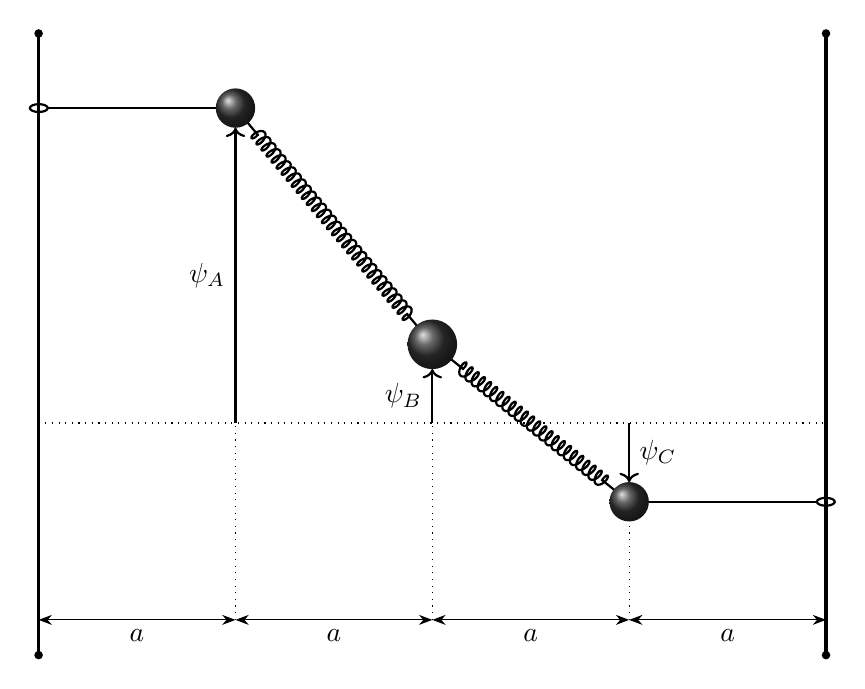
\begin{tikzpicture}
\coordinate (A) at (-2.5,4);
\coordinate (B) at (0,1);
\coordinate (C) at (2.5,-1);

\draw[very thick,{Circle[length=3pt]}-{Circle[length=3pt]}](-5,-3)--(-5,5);
\draw[very thick,{Circle[length=3pt]}-{Circle[length=3pt]}](5,-3)--(5,5);

\draw[thick,decoration={coil,aspect=-.5,post length=0.35cm,segment length=1mm,pre length=0.5cm},decorate](B)--(A);
\draw[thick,decoration={coil,aspect=-.5,post length=0.35cm,segment length=1mm,pre length=0.5cm},decorate](B)--(C);
\draw[thick,{Ellipse[open]}-](-5.125,0|-A)--(A);
\draw[thick,{Ellipse[open]}-](5.125,0|-C)--(C);

\draw[dotted](-2.5,-2.5)--(A);
\draw[dotted](0,-2.5)--(B);
\draw[dotted](2.5,-2.5)--(C);

\draw[dotted](-5,0)--(5,0);

\shade[ball color=black!80](A)circle(0.25);
\shade[ball color=black!80](B)circle(0.315);
\shade[ball color=black!80](C)circle(0.25);

\draw[{Stealth[]}-{Stealth[]}](-5,-2.5)--node[anchor=north]{$a$}(-2.5,-2.5);
\draw[{Stealth[]}-{Stealth[]}](-2.5,-2.5)--node[anchor=north]{$a$}(0,-2.5);
\draw[{Stealth[]}-{Stealth[]}](0,-2.5)--node[anchor=north]{$a$}(2.5,-2.5);
\draw[{Stealth[]}-{Stealth[]}](2.5,-2.5)--node[anchor=north]{$a$}(5,-2.5);

\draw[thick,->](-2.5,0)--node[anchor=east]{$\psi_A$}($(A)-(0,0.25)$);
\draw[thick,->](0,0)--node[anchor=east]{$\psi_B$}($(B)-(0,0.315)$);
\draw[thick,->](2.5,0)--node[anchor=west]{$\psi_C$}($(C)+(0,0.25)$);


\end{tikzpicture}
\end{document}